\chapter{Contribuciones}
\label{ch:contribuciones}

%* Comprobar
Durante el proceso de diseño del sistema de la FPGA, y ante la necesidad de crear módulos o bloques funcionales de utilidad en lenguaje Verilog\cite{stuartsutherland2001}, se siguen una serie de procedimientos definidos desde un comienzo. Gracias a su uso, a parte de establecer unos mínimos requerimientos de calidad, se obtienen con mayor eficiencia los resultados buscados, permitiendo a su vez una alta legibilidad del código, y una buena capacidad de modificación y reutilización.

Para garantizarlo, estos procedimientos deben de ser comunes en todos los módulos, e invariables a lo largo del proyecto.



%* Comprobar
\section{Etapas de diseño de un módulo}
\label{ch:contribuciones:etapas}
%* Comprobar
En primer lugar, tras requerir la utilización de un módulo que logre una función específica, se analiza la posibilidad de reutilizar uno o varios módulos anteriormente realizados, evitando así un derroche innecesario de tiempo y recursos.

%* Comprobar
Seguidamente, se estudia la complejidad del módulo a desarrollar, dividiendolo, si fuera necesario, en varios submódulos con funciones más concretas que disminuyan el grado de dificultad general en su elaboración, permitiendo a su vez una mayor reutilización futura de código.

%* Comprobar
Estando definida ya su distribución, se realiza un pequeño esquema sobre el que partir, que de forma gráfica muestre sus diversas partes y relaciones, junto a este, si fuera necesario, se dibuja otro que muestre las etapas de la máquina de estados, pudiendo a continuación empezar con la programación del mismo.

Cada módulo dispone de un estilo común, distribuido de la siguiente forma:
\begin{enumerate}
    %* Comprobar
    \item{\textbf{Comentario de cabecera.}} \\
    Tal como se muestra en el listado~\ref{src:metodologia-verilog-cabecera}, se nombra al módulo, incluyendo una descripción breve de sus funciones. Además, se enumeran y explican todas las entradas, salidas, parámetros y estados de los que está formado.
    \begin{lstlisting}[language=Verilog,
        caption={Ejemplo de comentario de cabecera del módulo.},
        label=src:metodologia-verilog-cabecera]
/*
 * <Nombre del modulo> module
 * <Descripcion del modulo>
 *
 * Parameters:
 *  - <Nombre del parametro>. <Descripcion del parametro>
 *  - etc ..
 *
 * Inputs:
 *  - <Nombre de la entrada>. <Descripcion de la entrada>
 *  - etc ..
 *
 * Outputs:
 *  - <Nombre de la salida>. <Descripcion de la salida>
 *  - etc ..
 *
 * States:
 *  - <Nombre del estado>. <Descripcion del estado>
 *  - etc ..
 */
    \end{lstlisting}

    %* Comprobar
    \item{\textbf{Control de reinicio síncrono/asíncrono (listado~\ref{src:metodologia-verilog-sync}).}} \\
    Se trata de un pequeño bloque que controla la forma de funcionamiento de los reinicios. Si en el archivo principal se define la constante \emph{ASYNC\_RESET}, entonces todos los reinicios serán asíncronos, en caso contrario, serán síncronos a la señal de reloj (\emph{clk}).
    \begin{lstlisting}[language=Verilog,
        caption={Ejemplo de control de reinicio síncrono/asíncrono.},
        label=src:metodologia-verilog-sync]
// X es el nombre del modulo en cada caso
`ifdef ASYNC_RESET
    `define X_ASYNC_RESET or negedge rst
`else
    `define X_ASYNC_RESET
`endif
    \end{lstlisting}
        
    %* Comprobar
    \item{\textbf{Incorporación de módulos necearios (listado~\ref{src:metodologia-verilog-include-modules}).}} \\
    Suele ser habitual, que el módulo que se está desarrollando haga uso de otros, los cuales son incorporar en este momento.
    \begin{lstlisting}[language=Verilog,
        caption={Ejemplo de incorporación de módulos.},
        label=src:metodologia-verilog-include-modules]
`include "./modules/nombre_del_modulo.vh"
\\ etc ..
    \end{lstlisting}
        
    %* Comprobar
    \item{\textbf{Creación del módulo (listado~\ref{src:metodologia-verilog-create}).}} \\
    Se define el módulo, agrupando las entradas y salidas según características similares, posicionando en primer lugar las entradas, seguido de las salidas.
    \begin{lstlisting}[language=Verilog,
        caption={Ejemplo de creación de módulo.},
        label=src:metodologia-verilog-create]
module nombre_modulo
    #(
      parameter nombre_parametro = valor_parametro
      \\ etc ..
     )
     (
      // <Nombre del primer grupo de entradas/salidas>
      input  wire nombre_entrada_1, // <breve descripcion>
        // etc ..
      output wire nombre_salida_1,  // <breve descripcion>
        // etc ..
     );
    \end{lstlisting}
    
    %* Comprobar
    \item{\textbf{Inicialización de módulos necesarios (listado~\ref{src:metodologia-verilog-mod-init}).}} \\
    Todos los módulos incorporados previamente necesitan ser inicializados, relacionando sus entradas/salidas con el resto de señales del módulo.
    \begin{lstlisting}[language=Verilog,
        caption={Ejemplo inicialización de módulos.},
        label=src:metodologia-verilog-mod-init]
// Ejemplo inicializando el modulo clk\_baud\_pulse, que tiene dos parametros, una entrada y dos salidas
clk_baud_pulse #(
                 .COUNTER_VAL(BAUDS),
                 .PULSE_DELAY(BAUDS/2)
                )
   clk_baud_Rx  (
                 .clk_in(clk),       // Input
                 .clk_pulse(clk_Rx), // Output
                 .enable(enable)     // Output
                );
    \end{lstlisting}
    
    %* Comprobar
    \item{\textbf{Creación de los registros de control (listado~\ref{src:metodologia-verilog-regs}).}} \\
    Se crean todos los registros encargados de controlar el módulo o almacenar las variables.
    \begin{lstlisting}[language=Verilog,
        caption={Ejemplo de creación de registros.},
        label=src:metodologia-verilog-regs]
// Control registers
reg [1:0]X_state_r   = 2'b0; // Register that stores the current X state
reg [3:0]X_counter_r = 4'b0; // Register that counts ...
reg [7:0]DATA_buff   = 8'b0; // Buffer where ...
    \end{lstlisting}

    %* Comprobar
    \item{\textbf{Creación de \textit{flags} o señales de control (listado~\ref{src:metodologia-verilog-flags}).}} \\
    Para poder identificar con facilidad si el sistema se encuentra en un estado concreto, se crean estas señales, cuyo valor será \textit{1} cuando la máquina de estados esté en dicho estado, y \textit{0} en caso contrario.
    \begin{lstlisting}[language=Verilog,
        caption={Ejemplo de creación de \textit{flags}.},
        label=src:metodologia-verilog-flags]
// Flags
wire X_s_IDLE; // HIGH if X\_state\_r == X\_IDLE, else LOW
wire X_s_RUN;  // HIGH if X\_state\_r == X\_RUN,  else LOW
    \end{lstlisting}

    %* Comprobar
    \item{\textbf{Asignación de valores de salida y señales internas (listado~\ref{src:metodologia-verilog-asignacion}).}} \\
    Se asignan los valores que tomarán los diversos \emph{wires}, tanto de uso interno, como de salida, estos pueden relacionarse con registros, salidas de módulos ya inicializados u otros \emph{wires}. Además, al final de cada asignación, se comenta cual va a ser su uso, por ejemplo, una asignación de salida o control.
    \begin{lstlisting}[language=Verilog,
        caption={Ejemplo de asignación de valores.},
        label=src:metodologia-verilog-asignacion]
// Assigns
assign X_s_IDLE = (X_state_r == X_IDLE) ? 1'b1 : 1'b0; // \#FLAG
assign X_s_RUN  = (X_state_r == X_RUN)  ? 1'b1 : 1'b0; // \#FLAG

assign nombre_salida_1 = DATA_buff[2]; // \#OUTPUT
    \end{lstlisting}
    

    %* Comprobar 
    \item{\textbf{Enumeración de estados (listado~\ref{src:metodologia-verilog-estados}).}} \\
    Se crean tantos parámetros locales como estados tenga el módulo, cada uno con un valor identificativo único.
    \begin{lstlisting}[language=Verilog,
        caption={Ejemplo de enumeración de estados.},
        label=src:metodologia-verilog-estados]
/// X States (See module description at the beginning of this file to get more info)
localparam X_IDLE = 1'b0;
localparam X_RUN  = 1'b1;
    \end{lstlisting}
    

    %* Comprobar
    \item{\textbf{Máquina de estados (listado~\ref{src:metodologia-verilog-fst}).}} \\
    Se fijan y distribuyen los diversos caminos que puede tomar el sistema. Para ello se realiza una máquina de estados \emph{Mealy}\cite{mealy1955method}, es decir, los nuevos estados dependen de las entradas y del propio estado actual. Un pequeño ejemplo de una máquina de estados se muestra en el listado \ref{src:metodologia-verilog-fst}
    \begin{lstlisting}[language=Verilog,
        caption={Ejemplo de máquina de estados.},
        label=src:metodologia-verilog-fst]
always @(posedge clk `X_ASYNC_RESET) begin
    if(!rst) X_state_r <= X_IDLE;
    else begin
        case(X_state_r)
            X_IDLE: begin
                if(!nombre_entrada_1) X_state_r <= X_RUN;
                else                  X_state_r <= X_IDLE;
            end
            X_RUN: begin
                X_state_r <= X_IDLE;
            end
            default: X_state_r <= X_IDLE;
        endcase
    end
end
    \end{lstlisting}

    %* Comprobar
    \item{\textbf{Actualización de registros (listado~\ref{src:metodologia-verilog-act-regs}).}} \\
    Por último, se actualizan los valores de los registros del módulo, teniendo en cuenta que se trata de una máquina de estados \emph{Mealy}\cite{barkalov2005design}.
    \begin{lstlisting}[language=Verilog,
        caption={Ejemplo de actualización de registros.},
        label=src:metodologia-verilog-act-regs]
always @(posedge clk `UART_RX_ASYNC_RESET) begin
    if(!rst) begin
        X_counter_r <= 0;
    end
    else if(X_s_IDLE) begin
        X_counter_r <= X_counter_r - 1'b1;
    end
    else if(X_s_RUN) begin
        X_counter_r <= X_counter_r + 1'b1;
    end
end
    \end{lstlisting}
\end{enumerate}



%* Comprobar
\section{Pruebas y simuaciones}
\label{ch:contribuciones:pruebas}
%* Comprobar
Para asegurar el correcto funcionamiento de cada módulo, estos deben superar varias pruebas que comprueben cada una de sus funcionalidades. En caso de superar todas ellas satisfactoriamente, el módulo estaría listo para ser usado en la síntesis de la FPGA, en caso contrario, tendría que volver a la fase de desarrollo, en la que buscar y solventar los fallos, utilizando los resultados de las simulaciones realizadas.

%* Comprobar
Estás pruebas hacen uso de las herramientas de código abierto \emph{Icarus Verilog}\footnote{Véase su repositorio: \url{https://github.com/steveicarus/iverilog}} (abreviado \emph{iverilog}), encargada de simular el propio código de \emph{Verilog}, y el visor de ondas \emph{GTKWave}\cite{gtkwave2019}, permitiendo generar y mostrar gráficamente todas las señales del circuito en cualquier instante de tiempo.

%* Comprobar
Para llevar a cabo dicha simulación, \emph{Iverilog} tiene como entrada un archivo en lenguaje \emph{Verilog} en el que se inicializa el propio módulo a analizar, y seguidamente, en ese mismo archivo, se van variando las entradas al módulo según su instante de tiempo. Posteriormente, y tras obtener el archivo con el resultado de la simulación, se abre en \emph{GTKWave} y se compara el resultado generado en el módulo, respecto al esperado.

En la figura~\ref{fig:ej-gtkwave} se muestra el resultado gráfico de una simulación de ejemplo.

\begin{figure}[htb]
    \centering
    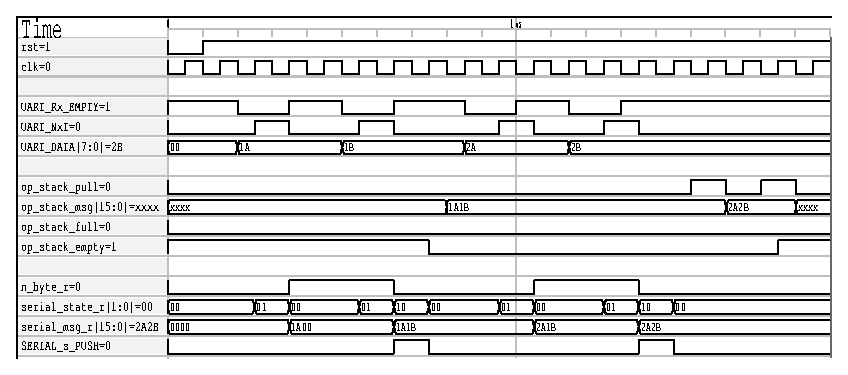
\includegraphics[width=120mm]{otro/ej_simulacion_gtkwave.eps}
    \caption{Ejemplo del resultado de una simulación en \emph{GTKWave}.}
    \label{fig:ej-gtkwave}
\end{figure}


%* Comprobar
\section{Distribución de archivos}
\label{ch:contribuciones:archivos}
Todo el código fuente utilizado por el sistema de la FPGA sigue una estructura concreta, reflejada en la figura~\ref{fig:tree-fpga}.
\begin{figure}[hbtp]
    \centering
    \begin{minipage}{11cm}
        \dirtree{%
            .1 ./.
            .2 modules/     \ldots{}
                            \begin{minipage}[t]{7cm}
                                \begin{flushright}
                                    Carpeta que contiene todos los módulos diseñados
                                \end{flushright}
                            \end{minipage}.
            .3 modulo\_1/.
            .4 rtl/.
            .4 tb/.
            .3 modulo\_2/.
            .4 rtl/.
            .4 tb/.
            .3 modulo\_1.vh     \ldots{}
                                \begin{minipage}[t]{6cm}
                                    \begin{flushright}
                                        Cada módulo diseñado debe tener un archivo de cabecera utilizado para inicializarlo
                                    \end{flushright}
                                \end{minipage}.
            .3 modulo\_2.vh.
            .3 ....
            .2 modules\_simulation/     \ldots{}
                                        \begin{minipage}[t]{5.2cm}
                                            \begin{flushright}
                                                Módulos usados unicamente en la simulación
                                            \end{flushright}
                                        \end{minipage}.
            .3 SB\_PLL40\_CORE.
            .3 SB\_RAM40\_4K/.
            .3 SB\_PLL40\_CORE.vh.
            .3 SB\_RAM40\_4K.vh.
            .2 rtl/     \ldots{}
                        \begin{minipage}[t]{7cm}
                            \begin{flushright}
                                Archivos principales del sistema
                            \end{flushright}
                        \end{minipage}.
            .3 bauds.vh/.
            .3 top.pcf/     \ldots{}
                            \begin{minipage}[t]{6.6cm}
                                \begin{flushright}
                                    Archivo que une los pines físicos con la lógica interna
                                \end{flushright}
                            \end{minipage}.
            .3 top.v/       \ldots{}
                            \begin{minipage}[t]{7cm}
                                \begin{flushright}
                                    Archivo Verilog principal
                                \end{flushright}
                            \end{minipage}.
            .2 tb/.
            .3 top\_tb.v/       \ldots{}
                                \begin{minipage}[t]{6.5cm}
                                    \begin{flushright}
                                        Archivo que simula el sistema en su conjunto
                                    \end{flushright}
                                \end{minipage}.
            .2 Makefile     \ldots{}
                            \begin{minipage}[t]{7cm}
                                \begin{flushright}
                                    Archivo de automatización de tareas
                                \end{flushright}
                            \end{minipage}.
        }
    \end{minipage}
    \caption{Estructura de carpetas del código de la FPGA}
    \label{fig:tree-fpga}
\end{figure}


% \chapter{Contribuciones}
% \label{ch:contribuciones-plantilla}

% Tus contribuciones no tienen por qué limitarse al trabajo sistemático del TFG.  Puede que hayas contribuido en aspectos metodológicos, en ideas novedosas, en la planificación de experimentos, en desarrollos matemáticos.

% Este capítulo está para agrupar todo eso.  Describe con claridad, y sin suponer conocimiento previo del desarrollo del proyecto (que viene después) todo lo que ha supuesto contribuciones originales por tu parte.